\subsection{Amortización y depreciación}

\subsubsection{Préstamo}

Para el inicio del proyecto se genero un préstamo con una entidad bancaria, el cual fue sumado al aporte social. En la tabla \ref{prestamo} se invierte en los activos fijos iniciales del proyecto y bajo que condiciones.

\vspace{2mm}
\begin{minipage}{0.9\textwidth}
\centering
\captionof{table}[{Préstamo}]{ Préstamo }
\label{prestamo}
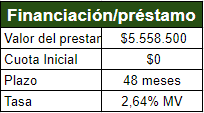
\includegraphics[\textwidth]{Images/prestamo.png}
\fnote{Nota. \textup{Fuente : Autores}}
\end{minipage}

\subsubsection{Amortización}

Se genera un resumen del pago realizado anualmente, en la tabla \ref{amortizacion} se evidencia la amortización total de la duda que se realiza en 4 años, de forma que, se observe como se pagara la deuda dentro del periodo de tiempo establecido y con qué saldo final terminara para llegar a 0, teniendo en cuenta intereses. 

\vspace{2mm}
\begin{minipage}{0.9\textwidth}
\centering
\captionof{table}[{Amortización}]{ Amortización }
\label{amortizacion}
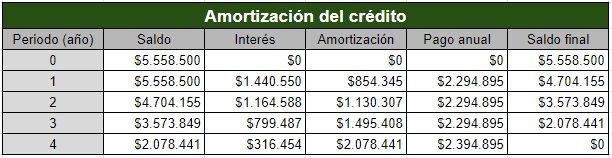
\includegraphics[width=0.9\textwidth]{Images/amortizacion.png}
\fnote{Nota. \textup{Fuente : Autores}}
\end{minipage}


\subsubsection{Depreciación}

En la tabla \ref{depreciacion} se considera la maquinaria que se va usar junto con su depreciación a partir del uso y obsolescencia de los dispositivos. Se calcula alrededor del 20\% depreciado de acuerdo a 5 años de vida útil.


\vspace{2mm}
\begin{minipage}{0.9\textwidth}
\centering
\captionof{table}[{Depreciación}]{ Depreciación }
\label{depreciacion}
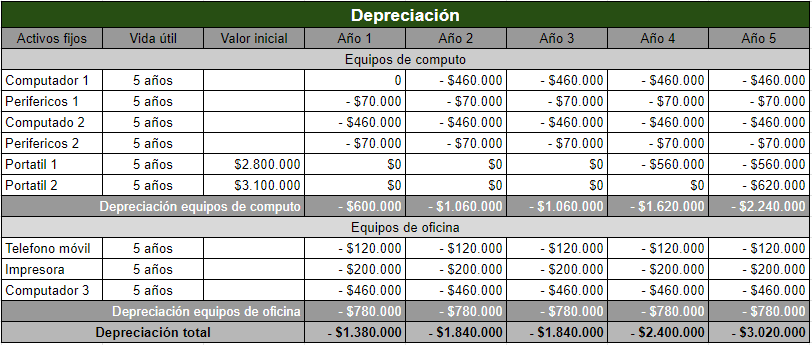
\includegraphics[width=0.9\textwidth]{Images/depreciacion.png}
\fnote{Nota. \textup{Fuente : Autores}}
\end{minipage}